\clearpage
\section{Linear Quadratic Regulator กับ Path Planning}
ในการทดลองครั้งนี้จะนำตัวควบคุม LQR ที่ได้ทำการทดลองหาค่าน้ำหนักที่ $Q$ กับ $R$ เหมาะสมจากการทดลองในบทก่อนหน้านี้มาทำการรวมกับ Path planning
เพื่อทำทดลองว่า Quadrotor สามารถบินไปตามตำแหน่งต่างๆตามที่ Path planning สั่งได้

ทำการสร้างเส้นทางที่เป็นรูปดาวด้วย Path Planning
\begin{figure}[!ht]
	\centering
	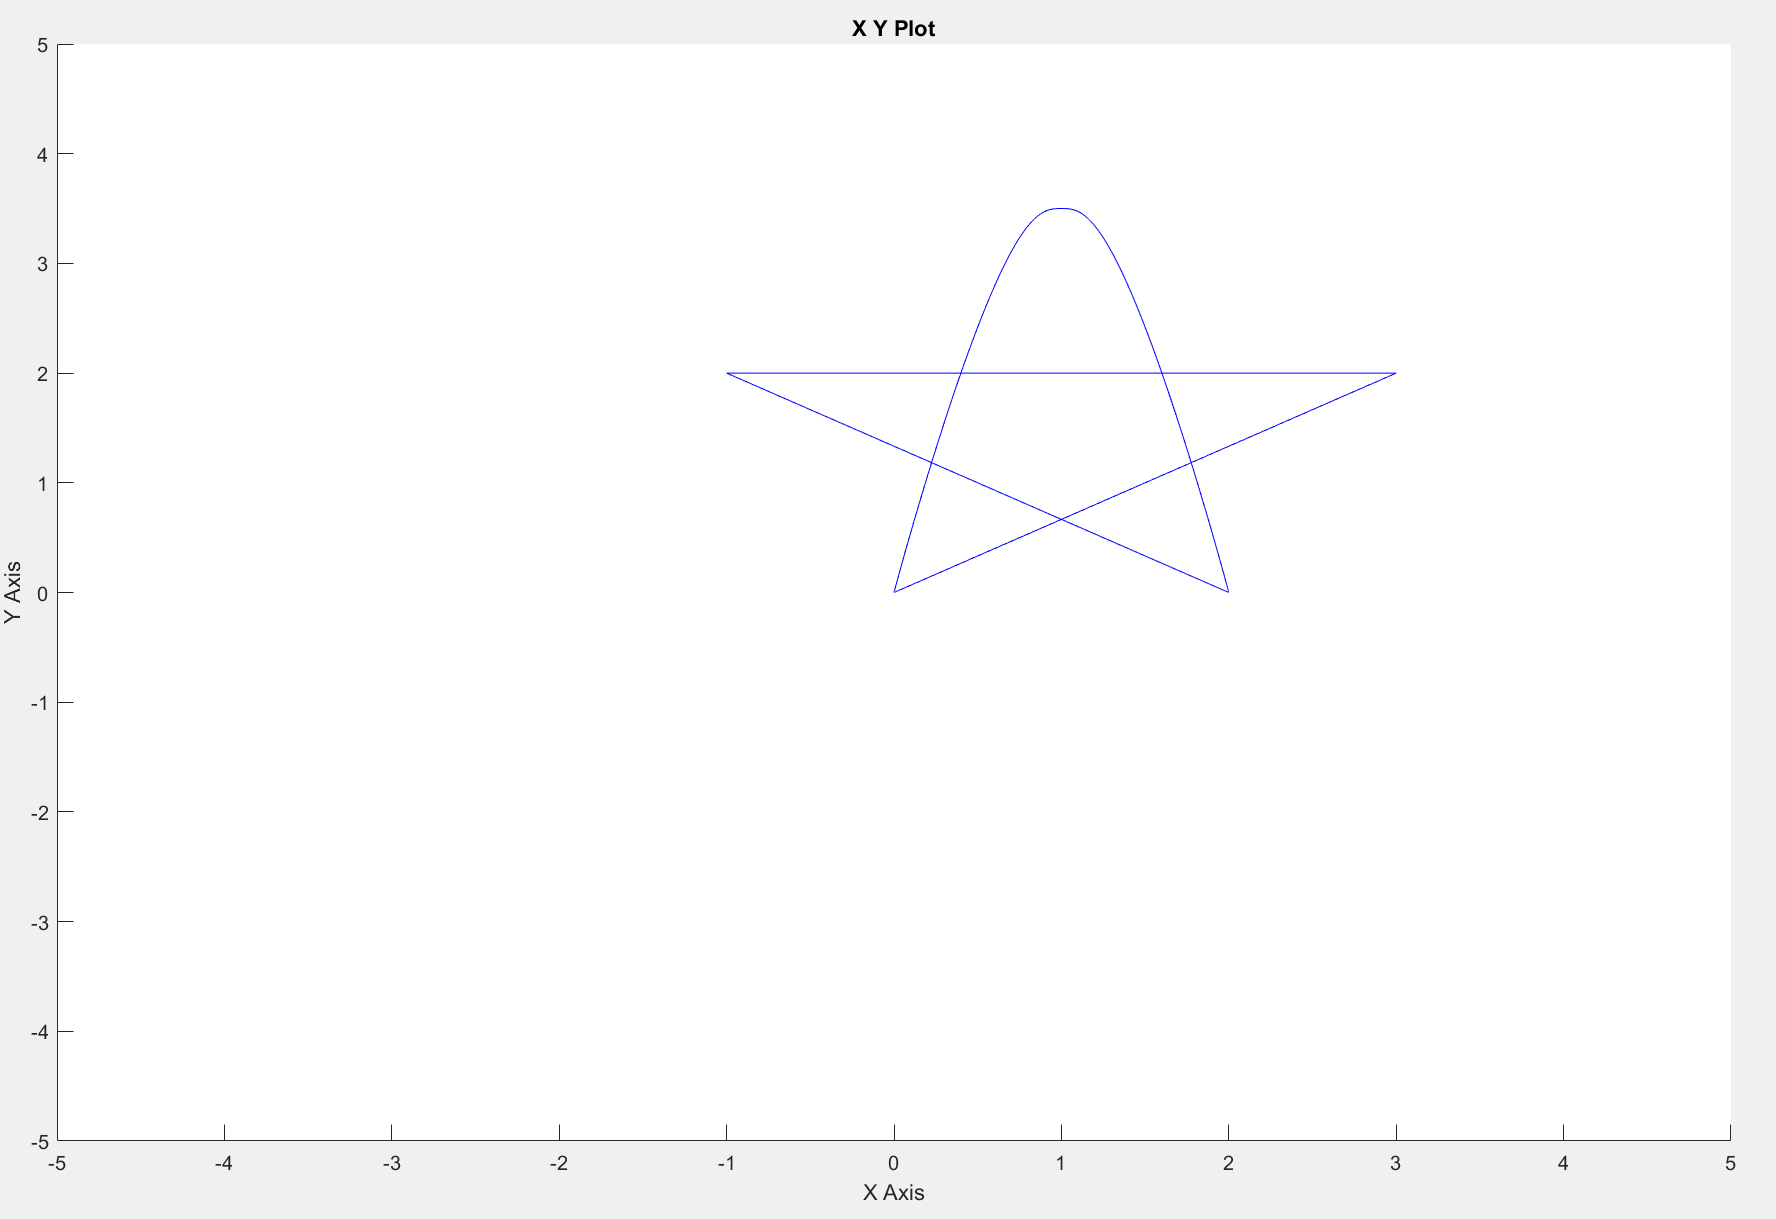
\includegraphics[width=0.8\textwidth]{images/simulink/star.png}
	\caption{เส้นทางของการวิ่งรูปดาว}
\end{figure}
\begin{figure}[!ht]
	\centering
	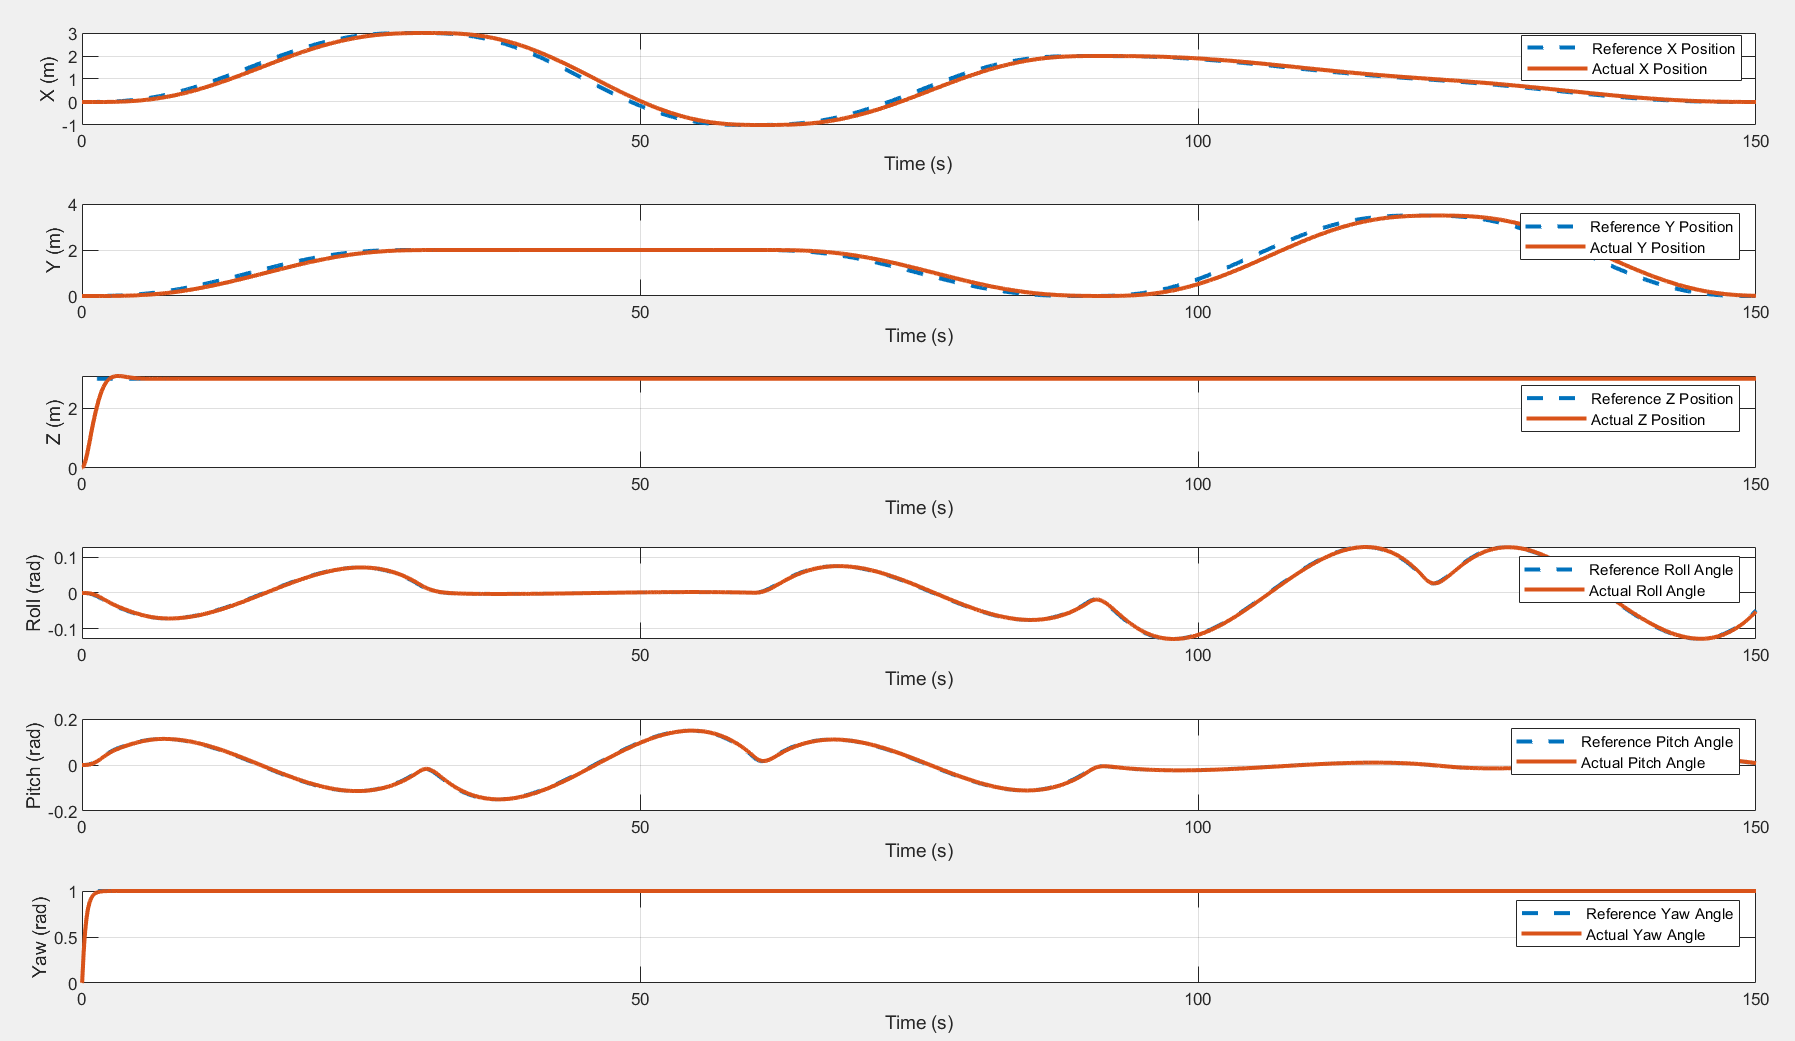
\includegraphics[width=0.8\textwidth]{images/simulink/simulation_star.png}
	\caption{สถานะQuadrotor ของการบินเป็นรูปดาว}
\end{figure}

จากกราฟจะได้เห็นว่า Quadrotor สามารถบินไปตามตำแหน่ง และ ทิศทางการหมุนตามที่ต้องการได้